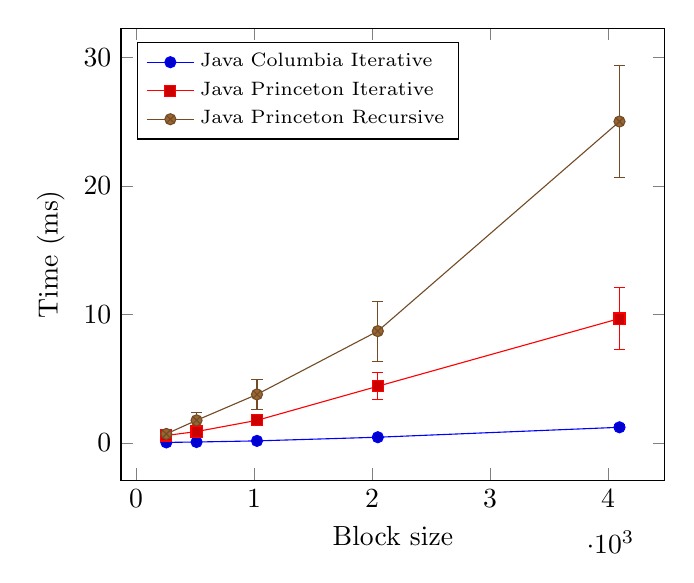
\begin{tikzpicture}
\begin{axis}[xlabel={Block size},ylabel={Time (ms)},width=0.70\linewidth,legend pos=north west,scaled x ticks={base 10:-3},legend cell align=left,legend style={font=\scriptsize}]
\addplot+[error bars/.cd, y dir=both,y explicit] coordinates {
(256, 0.0293) +- (0.0042, 0.0042)
(512, 0.0615) +- (0.0047, 0.0047)
(1024, 0.1484) +- (0.0308, 0.0308)
(2048, 0.4338) +- (0.0806, 0.0806)
(4096, 1.2071) +- (0.1807, 0.1807)
};
\addplot+[error bars/.cd, y dir=both,y explicit] coordinates {
(256, 0.5698) +- (0.4834, 0.4834)
(512, 0.8758) +- (0.3145, 0.3145)
(1024, 1.7488) +- (0.3452, 0.3452)
(2048, 4.4055) +- (1.0527, 1.0527)
(4096, 9.6792) +- (2.3947, 2.3947)
};
\addplot+[error bars/.cd, y dir=both,y explicit] coordinates {
(256, 0.6929) +- (0.1662, 0.1662)
(512, 1.7515) +- (0.6352, 0.6352)
(1024, 3.7688) +- (1.1879, 1.1879)
(2048, 8.6983) +- (2.3341, 2.3341)
(4096, 25.0276) +- (4.3322, 4.3322)
};
\legend{Java Columbia Iterative , Java Princeton Iterative , Java Princeton Recursive}
\end{axis}
\end{tikzpicture}
